
%%%%%%%%%%%%%%%%%%%%%%%%%%%%%%%%%%%%%%%%%%%%%%%%%%%%%%%%%%%%%%%%%%%%%%%%%%%%%%%%
%%%%%%%%%%%%%%%%%%%%%%%%%%%%%%%%%%%%%%%%%%%%%%%%%%%%%%%%%%%%%%%%%%%%%%%%%%%%%%%%
% STATE OF THE ART %
%%%%%%%%%%%%%%%%%%%%%%%%%%%%%%%%%%%%%%%%%%%%%%%%%%%%%%%%%%%%%%%%%%%%%%%%%%%%%%%%

\chapter{State of the art}
\label{chap:state}

In this chapter, the main technologies and tools used in the development of the project are described. Due to this work is composed of several different phases, the technologies utilized belong to different fields. For this reason, the definition of each of them will be categorized in the each of the described phases of the project. Figure~\ref{fig:phasesdistribution} presents the distribution of the phases throughout the project and the technologies used in each of them. 

 \begin{figure}
    \centering
    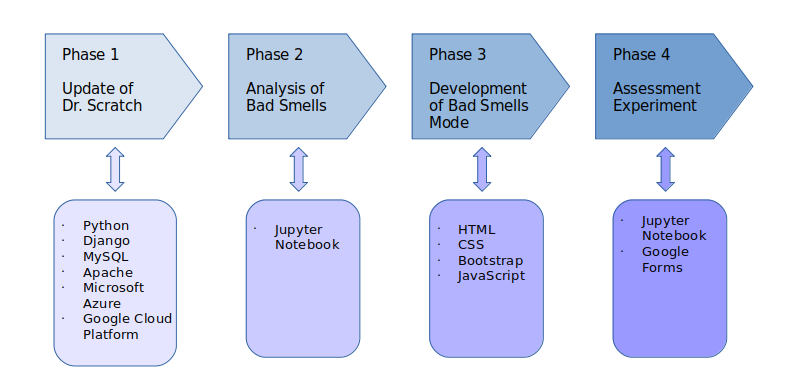
\includegraphics[width=15cm,keepaspectratio]{img/phases_state_art.png}
    \caption{Distribution of the technologies for each phase of the project.}
    \label{fig:phasesdistribution}
\end{figure}

\section{Phase 1. Update of the Dr. Scratch tool}
\label{sec:phase_1}

\subsection{Python} 
\label{subsec:python}

Python\footnote{https://www.python.org/} is a high-level general purpose computer programming language, suitable for web application implementation~\cite{kuhlman:python}. It is an open source language, optimized for software quality, developer productivity, program portability and component integration. Thanks to its characteristics, Python is used by hundreds of thousands of developers around the world and considered to be among the top four of five most widely-used programming languages in the world~\cite{lutz:programming}. The code of Dr. Scratch is programmed with the version 2.7 of the Python language. Some of its main features are as follows~\cite{javatpoint:_python}:

\begin{itemize}
  \item Easy to learn and use. Python is developer-friendly and high level programming language.
  
  \item Expressive language. Python is understandable and readable.
  
  \item Interpreted language. Python executes the code line by line at a time. This makes debugging easy and thus suitable for beginners.
  
  \item Cross-platform language. Python can run equally on different platforms such as Windows, Linux, Unix and Macintosh, among others. So, Python can be considered as a portable language.
  
  \item Object-Oriented language. Python supports object oriented language and concepts of classes and objects come into existence.
  
  \item Extensible. It implies that other languages such as C/C++ can be used to compile the code and thus it can be used further in our python code.
  
  \item Integrated. It can be easily integrated with languages like C, C++, JAVA, among others.
  
  \item Large standard library.
  
\end{itemize}



\subsection{Django}
\label{subsec:django}

Django\footnote{https://docs.djangoproject.com/} is a free and open source web application framework, written in Python. A web framework is a set of components that helps you to develop websites faster and easier~\cite{djangogirls}. Django was designed to help developers take applications from concept to completion as quickly as possible. There is an excellent documentation with several tutorials, guides or models about Django.

Django is based on the MVC pattern (Model-View-Controller), a software architecture pattern that separates data presentation from the logic of handling user interaction. The model handles data representation. It is defined in models.py and it serves as an interface to the data stored. Views represents the answer generated by a controller, commonly the HTML of a web page. Controller provides the logic and is composed by two scripts: urls.py, which manages the petitions to different views, and views.py, which generates the HTTP response. 

In this work, the versions implemented in the Dr. Scratch tool were 1.7 and 1.11 (Long-Term Support Release).


\subsection{MySQL}
\label{subsec:mysql}

MySQL\footnote{https://www.mysql.com/} is a Relational Database Management System (RDBMS) based on Structured Query Language (SQL). MySQL is based on a client-server model and the server, which is the core of MySQL, handles all of the instructions. The Dr. Scratch tool works with this database because it is associated with web applications and online tools. The main characteristics of MySQL are as follows:


\begin{itemize}
  \item MySQL is an open source software.
  \item High performance and scalability to meet the demands of growing data loads and users.
  \item Multi platform. Platform independence, giving you the flexibility to develop and deploy in multiple operating systems.
  \item Flexible and easy to use.
  \item High standard security.
\end{itemize}  

 

\subsection{Microsoft Azure}
\label{subsec:azure}

Microsoft Azure\footnote{https://portal.azure.com/} is a set of cloud services that allow to build, manage, and deploy applications on a global network using different tools and frameworks. Thanks to its online platform, it is easy to develop different services, such as computing, storage, analytical or networks. Dr.Scratch tool was hosted on a Virtual Machine, but the new version was migrated to another cloud service due to different reasons which will be detailed in Chapter~\ref{chap:implementation}. The Virtual Machines of Azure allow the implementation of tools and applications in a virtual system. Some of the reasons why Azure was chosen were:

\begin{itemize}
    \item Scalability. Possibility to personalize the required services in a Virtual Machine (type of machine, capacity, performance, etc.).
    \item Flexibility and payment for use. Easy deployment.
    \item Compatible with MySQL technology.
    \item High security.
\end{itemize}


\subsection{Apache}
\label{subsec:apache}

The Apache HTTP Server is a free and open source software web server. A server is necessary to show the content of the tool as a web page. Apache is a multi platform software, it works both in Unix and Windows servers. The server and the client communicate trough the HTTP protocol and Apache is the responsible for guaranteeing a fluency and safety communication between both extremes.

Apache is based on different modules and files that we had to configure to deploy the Dr. Scratch tool on the web. Thanks to its structure, it is highly personalized and we could host both versions in the domain. One of the most important modules is the mod\_wsgi module, which allows to connect Django and Azure. The current version that is working in Dr. Scratch is \textit{Apache/2.4.29}.  


\subsection{Google Cloud Platform}
\label{subsec:google}

Google Cloud Platform (GCP)\footnote{https://cloud.google.com/} is a set of physical resources, such as computers and hard disks, and virtual resources, such as Virtual Machines, which are in the data centers of Google around the world. The location of these data centers allows the distribution of the resources and consequently, a higher performance (because the services are closer to the clients).

There are a lot of available services in GCP, and the list is still growing. Thanks to its console, it is easy to manage and develop the necessary services for the tool Dr. Scratch. For that reason, among others, the new version was migrated from Azure to a new Virtual Machine of GCP. In Figure~\ref{fig:GCP}, we can observe the main console of GCP.

\begin{figure}
    \centering
        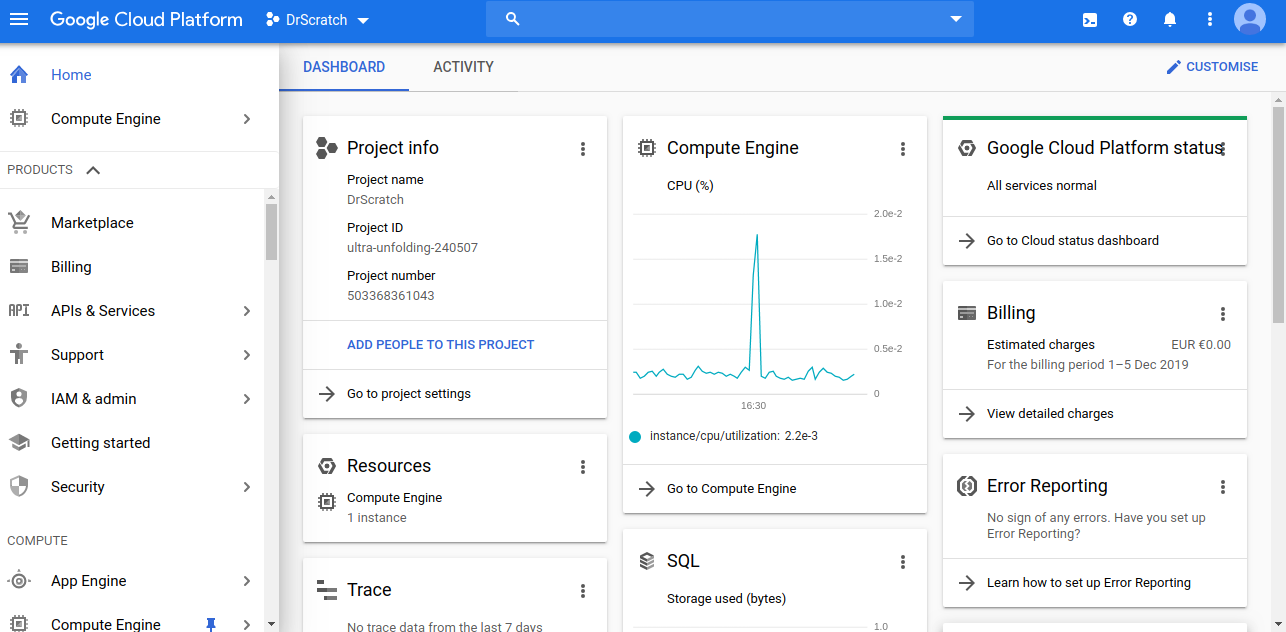
\includegraphics[width=11cm, keepaspectratio]{img/GCP.png}
        \caption{Dashboard of the Google Cloud Platform for the Dr. Scratch tool.}
        \label{fig:GCP}
\end{figure}



\section{Phase 2. Analysis of bad smells}
\label{sec:phase_2}

\subsection{Jupyter Notebook}
\label{subsec:jupyter}

Jupyter Notebook\footnote{https://jupyter.org/} is an interactive working environment which allows, in a dynamic way, the integration of Python code, text, graphics and pictures in the same document. It is useful for statistical analysis, machine learning, data management, etc. Some of the libraries which Jupyter includes and we have implemented in the analysis are:

\begin{itemize}
    \item \textit{Pandas}\footnote{https://pandas.pydata.org/} is an open source library which provides high-performance, easy-to-use data structures and data analysis for the Python language. Its primary data structure is \textit{DataFrame}, a potentially heterogeneous data structure with labeled axes (rows and columns). It has been essential for the management of the analyzed data set.
    \item \textit{NumPy} is the fundamental package for scientific computing. It contains a powerful N-dimensional array object, sophisticated functions, useful linear algebra, etc.
    \item The \textit{matplotlib.pyplot} library. It allows multiple options to work with graphics or figures. It is necessary to represent the data and results.
    \item The \textit{scipy.stats} module contains a large number of probability distributions as well as statistical functions. In particular, we have implemented in this study the t-student statistical analysis. 
\end{itemize}



\section{Phase 3. Development of bad smells model}
\label{sec:phase_3}

\subsection{HTML}
\label{subsec:html}

HTML (HyperText Markup Language) is a language designed for web tools. The first version of HTML was launched in 1991, by the British scientist Timohty John Berners-Lee and it contained few items. 

HTML is a language composed of different elements, tags and attributes. Thanks to its tree structure, it is possible to describe the content of a page in plane text. In the following example we can observe how the content is composed of opening tags, possible attributes and closing tags. 

{\footnotesize
\begin{verbatim}
    <!DOCTYPE html>
    <html>
        <head>
            <title> Dr. Scratch </title>
        </head>
        <body>
            <div id="myExample">
                <p> This is a paragraph </p>
            <div>
        </body>
    </html>        
\end{verbatim}
}

The first official standard HTML 2.0 was released in 1995. Actually, we have used the last version published in 2014, HTML 5. All the interface of Dr. Scratch is designed with templates of HTML.


\subsection{CSS}
\label{subsec:css}

CSS (Cascading Style Sheets) is a language used to define styles for web pages. Mainly, it is used to describe the style of HTML files, such as the design, colors or fonts. CSS has a simple syntax and it can control multiple pages all at once. The same way, CSS is composed of elements, tags and attributes. We can observe an example of its structure.  

{\footnotesize
\begin{verbatim}
    #example {
        height: 100%;
        margin: 0 -60px;
    } 
    
    body{
        font-family: sans-serif;
        background-color: red;
    }
\end{verbatim}
}

\subsection{Bootstrap}
\label{subsec:bootstrap}

Bootstrap\footnote{https://getbootstrap.com/} is an open source framework for developing with HTML, CSS, and JavaScript. It facilitates the design and appearance of the web tools by means of CSS libraries which include buttons, typography, menus, etc. Bootstrap is responsive, that is, it allows to adapt the web pages to any type of devices and screens.
In addition, the Bootstrap platform offers a good documentation and a large number of free templates with the implementation of the design of a complete web page. 


\subsection{JavaScript}
\label{subsec:javascript}

JavaScript is a programming language which works on the client side. It is an interpreted language, which means it can be incorporated in a web page without the need of compilation. JavaScript code runs directly in a web browser and it controls the dynamic elements of the web page. 

Although the JavaScript code can be in external files, usually it is located between the tags of the HTML document:
{\footnotesize
\begin{verbatim}
    <body>
        <script>
            JavaScript Code
        </script>        
    </body>
\end{verbatim}
}



\section{Phase 4. Assessment experiment}
\label{sec:phase_4}

\subsection{Google Forms}
\label{subsec:google_forms}

Google Forms\footnote{https://www.google.es/intl/es/forms/about/} is a tool which allows the creation of simple forms or questionnaires. It collects data from online surveys which can be obtained in data sheets. It is a way to gather information quickly and easily.

Thanks to this tool, it was possible to develop, in a simple way, some questionnaires for the different teacher profiles who implemented the experiment. We obtained different answers and data from Google Forms and then we could analyze them easily.


